\documentclass{article}
% --- Page Layout ---
\usepackage[a4paper, landscape, twocolumn, margin=1.5cm, columnsep=1cm]{geometry}
\usepackage[hidelinks]{hyperref}


% --- Text ---
\usepackage{ulem, multicol, afterpage, enumitem}
\let\oldemph\emph
\renewcommand{\emph}[1]{\textit{#1}}


% --- Code --- 
\usepackage{algpseudocodex}
\algrenewcommand\algorithmicforall{\textbf{for each}}


% --- Math ---
\usepackage{amsthm, amsmath, amsfonts, amssymb}
\numberwithin{equation}{section}
\usepackage{xcolor, tcolorbox}
\tcbuselibrary{theorems}


% --- Environments ---
\definecolor{darkgreen}{RGB}{19, 79, 25}

\newenvironment{pane}{
    \begin{tcolorbox}[left=5pt, right=5pt, center, colback=gray!5!white, colframe=gray!50]
}{
    \end{tcolorbox}
}

\newenvironment{myproof}[1]{
    \begin{tcolorbox}[colback=white, colframe=gray!50, title=\bfseries #1]
}{
    \end{tcolorbox}
}
\newenvironment{continueMyproof}{
    \begin{tcolorbox}[colback=white, colframe=gray!50]
}{
    \end{tcolorbox}
}

\newenvironment{definitions}{
    \begin{tcolorbox}[right=30pt, colback=darkgreen!9, colframe=darkgreen, title=\bfseries Definitions]
}{
    \end{tcolorbox}
}
\newenvironment{definition}[1]{
    \begin{tcolorbox}[colback=darkgreen!9, colframe=darkgreen, title=\bfseries Definition#1]
}{
    \end{tcolorbox}
}

\newenvironment{example}[1]{
    \begin{tcolorbox}[colback=blue!5!white, colframe=blue!75!black, title=\bfseries Example#1]
}{
    \end{tcolorbox}
}
\newenvironment{continueExample}{
    \begin{tcolorbox}[colback=blue!5!white, colframe=blue!75!black]
}{
    \end{tcolorbox}
}

\newenvironment{exercise}[1]{
    \begin{tcolorbox}[colback=white, colframe=gray!75!black, title=\bfseries Exercise#1]
}{
    \end{tcolorbox}
}
\newenvironment{continueExercise}{
    \begin{tcolorbox}[colback=white, colframe=gray!75!black]
}{
    \end{tcolorbox}
}


% --- Theorems & Definitions ---
%\renewcommand\qedsymbol{$\blacksquare$}
\newtcbtheorem{Definition}{Definition}
{colback=red!5!white, colframe=red!75!black, fonttitle=\bfseries}{}
\newtcbtheorem{Corollary}{Corollary}
{colback=purple!5!white, colframe=purple!80, fonttitle=\bfseries}{}
\newtcbtheorem{Theorem}{Theorem}
{colback=green!5!white, colframe=green!75!black, fonttitle=\bfseries}{}


% --- Graphics ---
\usepackage{graphicx}
\graphicspath{ {./images/} }
\usepackage{wrapfig}
\usepackage{tikz}

\author{Alessio Arcara, Alessia Crimaldi}
\begin{document}
\begin{titlepage}
    \vspace*{\fill}
	\centering
   	\Huge Languages and Algorithms for Artificial Intelligence\\
	\vspace{0.2cm}
   	\huge Module 2: Logic and Logic Programming\\
   	\vspace{0.7cm}
   	\Large Alessio Arcara $\qquad$ Alessia Crimaldi\\
   	\vspace{0.2cm}
   	\begin{center}
    	
\includegraphics[width=0.4\linewidth]{prolog_meme}
   	\end{center}
   	\vspace*{\fill}
\end{titlepage}
\pagenumbering{gobble}

\tableofcontents
\clearpage

\pagenumbering{arabic}
\parindent 0pt

\cleardoublepage

\section{Logic}
\paragraph{Truth.}
The notion of truth is always defined with respect to a world. The problem
is when the world changes or when we adopt new world; in such cases, the truth
also changes. Therefore, there isn't something that is universally true, and
it is better to replace it with the concept of logical consequence, which
doesn't change with the world. 

\begin{Definition}{Logical Consequence}{}
    For a set of sentences $\Gamma=F_1,\ldots,F_n$, we say that $F$ is a
    logical consequence of $\Gamma$ in various possible worlds, if it is
    always true that: whenever all sentences in $\Gamma$ are true, then $F$
    is true.
\end{Definition}
\begin{Definition}{Logical Equivalence}{}
    if $F$ is logical consequence of $G$ and $G$ is logical consequence of
    $F$, then they are equivalent.
\end{Definition}
Now, the notion of truth becomes contextual rather than universal, and the
world is characterized by the sentences that describe it.

\subsection{Propositional logic}
Propositional logic is the logic which deals only with propositions.
\begin{Definition}{Proposition}{}
    A proposition $P_i$ is a statement about some specific fact which can be true or
    false. $P_{i}$ is an atom or atomic formula.
\end{Definition}
\begin{example}
   \begin{itemize}
       \item Today it is raining
       \item I take the umbrella
       \item There is the sun
   \end{itemize}
\end{example}
We can build larger sentences from smaller ones by using \textbf{connectives}.
While natural language provides a rich source of connectives, we opt for
connectives that do not introduce confusion to build an unambiguous artificial
language. For the same reason, we do not use natural language because it is
ambiguous by its nature. Consequently, our goal is to build a precise
artificial language that is not ambiguous.
\begin{example}
    \begin{itemize}
        \item John drove on and hit a pedestrian.
        \item John hit a pedestrian and drove on.
        \item If I open the window then 1+3=4
    \end{itemize}
\end{example}
To do so, the logic, like any formal system, needs to define both
\textbf{syntax} and \textbf{semantics}. Syntax specify the rules which tell us
how the well formed sentences are constructed, while semantics specify the
rules which tell us the meaning of the well formed sentences.
\begin{Definition}{Alphabet}{}
    The language of propositional logic has an alphabet consisting of
    \begin{enumerate}
        \item proposition symbols: $p_0,p_1,\ldots$,
        \item connectives: $\land,\lor,\rightarrow,\neg,\leftrightarrow,\perp$,
        \item auxiliary symbols: $(,)$.
    \end{enumerate}
    The connectives carry traditional names:
    \begin{align*}
        \land & \quad \text{ - and} & \quad \text{ - conjunction} \\
        \lor & \quad \text{ - or} & \quad \text{ - disjunction} \\
        \rightarrow & \quad \text{ - if ..., then ...} & \quad \text{ - implication} \\
        \neg & \quad \text{ - not} & \quad \text{ - negation} \\
        \leftrightarrow & \quad \text{ - iff} & \quad \text{ - equivalence, bi-implication} \\
        \bot & \quad \text{ - falsity} & \quad \text{ - falsum, absurdum}
    \end{align*}
    The proposition symbols and $\perp$ stand for indecomposable propositions,
    which we call \textbf{atoms}, or \textbf{atomic propositions}.
\end{Definition}
\clearpage
Well-formed formula is defined recursively:
\begin{center}
    \begin{bnf}
        formula ::= Atomic Proposition
        | $\neg$ formula
        | formula $\land$ formula
        | formula $\lor$ formula
        | formula $\rightarrow$ formula
        | formula $\leftrightarrow$ formula
        | (formula)
    \end{bnf}
\end{center}
If we write the proposition ``Today it is raining" is it true or false? Of
course, as said in previous section, it depends on the world we are considering,
so we need the notion of \textbf{interpretation}.
\begin{Definition}{Interpretation}{}
    Given a formula $G$, let $\{A_1,\ldots,A_n\}$ be a set of atoms which
    occur in the formula, an interpretation $I$ of $G$ is an \underline{assignment of
    truth values} to $\{A_1,\ldots,A_n\}$.
\end{Definition}
The semantics of a formula are defined by the truth values of its atoms and
their corresponding connectives. We can represent each possible combination of
truth values in a structure format known as a \textbf{truth table}.
\begin{center}
    \begin{tabular}{@{ }c@{ }@{ }c | c@{ }c@{ }c@{ }c@{ }c@{ }}
        $p_1$ & $p_2$ & $\neg p_1$ & $p_1\land p_2$ & $p_1\lor p_2$ &
        $p_1\rightarrow p_2$ & $p_1\leftrightarrow p_2$\\
        \hline 
        T & T & F & T & T & T & T\\
        T & F & F & F & T & F & F\\
        F & T & T & F & T & T & F\\
        F & F & T & F & F & T & T\\
    \end{tabular}
\end{center}
It's important to note that implication can be a bit tricky: if $p_1$ is true,
then $p_2$ must also be true; however, if $p_1$ is false, any value is okay
for $p_2$.
\begin{exam}
Write the truth table for the formula $G=(P\lor Q)\land\neg(P\land Q)$:
    \begin{center}
        \begin{tabular}{@{ }c@{ }@{ }c | c@{ }c@{ }c@{ }c@{ }c@{ }}
            $P$ & $Q$ & $P\lor Q$ & $P\land Q$ &
            $\neg(P\land Q)$ & $G$ \\
            \hline 
            T & T & T & T & F & F & \\
            T & F & T & F & T & T & \\
            F & T & T & F & T & T & \\
            F & F & F & F & T & F & \\
        \end{tabular}
    \end{center}
\end{exam}
\begin{Definition}{Model}{}
    We say that an interpretation $INT$ is a model of a formula $F$, written
    $$INT\models F$$
    if $F$ is true when the truth value of propositional symbols is defined
    according to $INT$.
\end{Definition}
\begin{Definition}{Validity}{}
   A formula $F$ is valid iff it is true in all its interpretation. If $F$ is
   valid we can write $\models F$.
\end{Definition}
\begin{example}
   $A\lor\neg A$ is a valid formula.
\end{example}
\begin{Definition}{Satisfiability}{}
    A formula $F$ is satisfiable iff there exists an assignment of truth
    values that can make the formula true. If $F$ is satisfiable we can write
    $I\models F$.
\end{Definition}
\begin{example}
   $A\land\neg A$ is an unsatisfiable formula. 
\end{example}
\begin{Definition}{Decidability}{}
    \underline{Propositional logic is decidable}: there is a terminating
    procedure to check whether a formula is valid.

    The algorithm is simple: write down the complete truth table for the
    formula and check if the last column contains only $T$. Such algorithm has
    a computation cost of $2^n$, where $n$ is the number of interpretations.
\end{Definition}

\begin{Definition}{Logical Equivalence}{}
   Two formulas $F$ and $G$ are logically equivalent $F\equiv G$ iff the truth
   values of $F$ and $G$ are the same under every interpretation of $F$ and
   $G$.
\end{Definition}
\begin{center}
    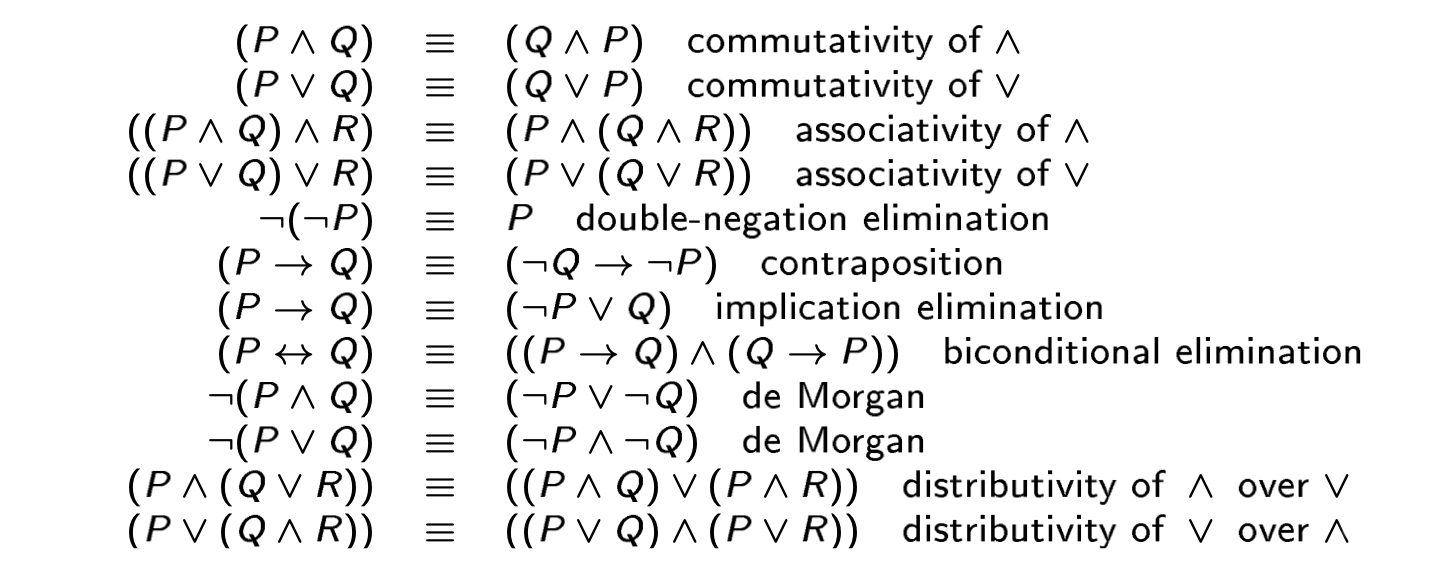
\includegraphics[width=\linewidth]{logical_equivalence}
\end{center}
\begin{Definition}{Literal}{}
   A literal is an atom or the negation of an atom.  
\end{Definition}
\begin{Definition}{Negation Normal Form (NNF)}{}
   A formula is in Negation Normal Form iif negations appears only in front
   of atoms.
\end{Definition}
\begin{Definition}{Conjunctive Normal Form (CNF)}{}
   A formula $F$ is in Conjunctive Normal Form iif it is in NNF and it has the
   form $F_1\land F_2\land\ldots\land F_n$ where each $F_i$ is a disjunction of
   literals.
\end{Definition}
\begin{example}
    $(\neg P\lor Q)\land(\neg P\lor R)$ is in CNF.\\
    $\neg(\neg P\lor Q)\land(\neg P\lor R)$ is not in CNF.
\end{example}
\begin{Definition}{Disjunctive Normal Form (CNF)}{}
   A formula $F$ is in Disjunctive Normal Form iif it is in NNF and it has the
   form $F_1\lor F_2\lor\ldots\lor F_n$ where each $F_i$ is a conjunction of
   literals.
\end{Definition}
\begin{example}
   $(\neg P\land R)\lor(Q\land\neg P)$ is in DNF.
\end{example}
Any formula can be transformed into a normal form by using the equivalence
rules. Normal form is easier to evaluate for a machine.
\begin{exam}
    Example of transformation in CNF
    $$
    \begin{aligned}
        (P\rightarrow Q)\land(R\lor(B\land A)) &\equiv \\ 
                                               &\equiv(\neg P\lor
                                               Q)\land(R\lor(B\land A))\\
                                               &\equiv (\neg P\lor
                                               Q)\land((R\lor B)\land (R\lor
                                               A))\\
                                               &\equiv (\neg P\lor
                                               Q)\land(R\lor B)\land (R\lor
                                               A)\\
    \end{aligned}
    $$
    Basically, we begin by applying implication elimination, followed by the
    pushing of negations within the formula. After that we apply the
    distribution of connectives.
\end{exam}
\begin{Definition}{Logical Consequence}{}
    Given a set of formulas $\{F_1,\ldots,F_n\}$ and a formula $G$, $G$ is
    said be a logical consequence of $F_1,\ldots,F_n$, denoted as
    $F_1\land\ldots \land F_n\models G$, iff for any interpretation $I$ in
    which $F_1\land\ldots\land F_n$ is true $G$ is also true.
\end{Definition}
Instead of constructing the truth table, the following theorems show that we
can prove logical consequence by proving validity of a formula or proving a
given formula is never satisfiable.
\begin{Theorem}{Deduction}{}
    Given a set of formulas $\{F_1,\ldots,F_n\}$ and a formula $G$,
    $F_1\land\ldots \land F_n\models G$ iif $\models(F_1\land\ldots F_n)\to G$
    (is valid).
\end{Theorem}
\begin{Theorem}{Refutation}{}
    Given a set of formulas $\{F_1,\ldots,F_n\}$ and a formula $G$,
    $(F_1\land\ldots\land F_n)\models G$  iif $F_1\land\ldots\land F_n\neg G$
    is never satisfiable.
\end{Theorem}
\begin{example}
    To determine if an argument is valid in propositional logic, the initial
    step is to identify the basic propositions from natural language and
    disregard anything irrelevant (e.g. quantifiers).

    All the dated letters in this room are  written on blue paper,

    This is decomposed as:
    \begin{itemize}
        \item $P$: the letter is dated; 
        \item $Q$: the letter is written on blue paper;
        \item $P\to Q$.
    \end{itemize}
    None of them are in black ink, except those that are written in third
    person.

    This is decomposed as:
    \begin{itemize}
        \item $S$: letters is written in the third person. 
        \item $R$: the letter is written in black ink.
        \item $\neg S\to\neg R$
    \end{itemize}
\end{example}
\begin{exam}
    If John drinks beer, he is at least 18 years old. John does not drink
    beer. Therefore, John is not yet 18 years old.

    \begin{itemize}
        \item $D$: John drinks beer 
        \item $Y$: John is at least 18 year old
        \item $\neg D$
        \item $D\to Y$
    \end{itemize}

    We want to prove that $D\to Y\land\neg D\models\neg Y$, assuming all the
    sentences are true. We can do this using three different methods:
    \begin{itemize}
        \item truth table
            \begin{center}
                \begin{tabular}{@{ }c@{ }@{ }c | c@{ }c@{ }c@{ }c}
                    $D$ & $Y$ & $\neg D$ & $D\to Y$ & $\neg D \land (D\to Y)$
                        & $\neg Y$ \\
                    \hline
                    T & T & F & T & F & F \\
                    T & F & F & F & F & T \\
                    F & T & T & T & T & F \\
                    F & F & T & T & T & T \\
                \end{tabular}
            \end{center}
        \item deduction: $\models(D\to Y\land \neg D)\to \neg Y$
        \item refutation: $D\to Y\land \neg D\land Y$ is never
            satisfiable
    \end{itemize}
\end{exam}
\subsection{Natural deduction}
We have seen a way to prove logical consequences based on semantics, using
truth tables. However, we can also prove logical consequences through syntax,
which is much more efficient. This involves performing syntactic manipulations
of the symbols through a sequence of steps. Each step represents a derivation
of a conclusion from the given premises. That can be expressed as:
$$
\begin{prooftree}
    \hypo{\text{premises}}
    \infer1{\text{conclusion}}
\end{prooftree}
$$
The derivation perform either elimination or introduction of connectives,
using the following derivation rules:
\begin{itemize}
    \item \textbf{Conjuction introduction}: if $A$ is true and $B$ is true we
        may conclude $A\land B$ is true.
        $$\begin{prooftree}
            \hypo{A}\hypo{B}
            \infer2[$\land I$]{A\land B}
        \end{prooftree}$$
    \item \textbf{Conjunction elimination}: if $A\land B$ is true we may
        conclude $A$ is true (or $B$ is true).
        $$\begin{prooftree}
            \hypo{A\land B}
            \infer1[$\land E$]{A}
        \end{prooftree}
        \quad\text{or}\quad
        \begin{prooftree}
            \hypo{A\land B}
            \infer1[$\land E$]{B}
        \end{prooftree}$$
    \item \textbf{Implication introduction}: if $B$ follows from $A$,
        then we may conclude $A\to B$. 
        $$\begin{prooftree}
            \hypo{[A]}
            \ellipsis{}{B}
            \infer1[$\to I$]{A\to B}
        \end{prooftree}$$
        Note that implication is only valid along the specific path of the
        proof tree. Once the implication is derived, the initial hypothesis
        becomes redundant and can be discarded (denoted as $[]$), as it is
        inherently contained within the implication.
    \item \textbf{Implication elimination}: if $A$ true and we know that $B$
        follows from $A$, then we have also $B$ is true.
        $$\begin{prooftree}
            \hypo{A}\hypo{A\to B}
            \infer2[$\to E$]{B}
        \end{prooftree}$$
    \item \textbf{Ex falso sequitur quodlibet}: if we have a false premise, we
        can derive any possible formula.
        $$\begin{prooftree}
            \hypo{\perp}
            \infer1[$\perp$]{A}
        \end{prooftree}$$
    \item \textbf{Reduction Ad Absurdum}: if one derives a contradiction from
        the hypothesis $\neg A$, then one has a derivation of $A$ (without the
        hypothesis $\neg A$).
        $$\begin{prooftree}
            \hypo{[\neg A]}
            \ellipsis{}{\perp}
            \infer1[RAA]{A}
        \end{prooftree}$$
\end{itemize}
In that process, a deduction tree is built. Each internal node represents a
derivation step, with the root corresponding to the formula, and the
hypotheses are the leaves of the tree.

We restrict our language to the connectives $\land,\to$ and $\perp$. Negation
can be express as $A\to\perp$.
\begin{example}
    $$\begin{prooftree}
        \hypo{A\land B} 
        \infer1[($\land E$)]{A}
        \hypo{C\land D} 
        \infer1[($\land E$)]{D}
        \infer2[($\land I$)]{A\land D}
    \end{prooftree}$$
\end{example}
\begin{example}
    Demonstrate commutativity $A \land B \to B \land A$  using only natural
    deduction
    $$\begin{prooftree}
        \hypo{[A\land B]^1}
        \infer1[$\land E$]{B}
        \hypo{[A\land B]^1}
        \infer1[$\land E$]{A}
        \infer2[$\land I$]{B\land A}
        \infer1[$\to I_1$]{A\land B\to B\land A}
    \end{prooftree}$$
    At last, it has been used the implication introduction and it has been
    discarded the hypothesis to prove that $B\to A$ is always true.
\end{example}
\begin{example}
   Provide the proof for $A\to\neg\neg A\equiv A\to\neg(A\to\perp)\equiv
   A\to((A\to\perp)\to\perp)$.
   $$
   \begin{prooftree}
       \hypo{[A]^2}\hypo{[A\to\perp]^1}
       \infer2[$\to E$]{\perp}
       \infer1[$\to I_1$]{((A\to\perp)\to\perp)}
       \infer1[$\to I_2$]{(A\to((A\to\perp)\to\perp)}
   \end{prooftree}
   $$
\end{example}
The derivation process serves the purpose to proving validity of a given
formula. However, when there is a suspect that a formula might be false, we
need to identify an assignment of truth values that makes the formula false.
\begin{Definition}{}{}
    We write $\Gamma\vdash\psi $ if there exists a deduction tree with the
    conclusion $\psi$ as the root and the premises $\Gamma$, which are not
    discarded, as the leaves.

    When $\Gamma=\emptyset$, so all premises are discarded, we say that $\psi$
    is a \textbf{theorem}.
\end{Definition}
\begin{Theorem}{Completeness}{}
   $$\Gamma\vdash\psi\Leftrightarrow\Gamma\models\psi$$
\end{Theorem}
This theorem tells us that what we derive is true, and all that is true can be
derived.
\begin{exam}
    $A\to(B\to C)\to(A\land B\to C)$

    To prove the validity of the given formula, we can use only the natural
    deduction method. The goal is to demonstrate the truth by discarding all
    the hypotheses in the deduction tree.

    Before proceeding with the proof, it's important to evaluate whether the
    given formula appears more reasonably true or false. Otherwise, we could
    spend half an hour proving the wrong thing.

    The formula provides us a strategy for tackling the problem. One approach
    can be to proceed backward to validate the formula:
    \begin{enumerate}
        \item $\begin{prooftree}
                \hypo{A\land B\to C}
                \infer1[$\to I$]{A\to(B\to C)\to(A\land B\to C)}
            \end{prooftree}$
        \item $\begin{prooftree}
                \hypo{C}
                \infer1[$\to I$]{A\land B\to C}
            \end{prooftree}$
        \item $\begin{prooftree}
                \hypo{B}\hypo{B\to C}
                \infer2[$\to E$]{C}
            \end{prooftree}$
            \begin{enumerate}
                \item $\begin{prooftree}
                        \hypo{A\land B}
                        \infer1[$\land E$]{B}
                    \end{prooftree}$
                \item $\begin{prooftree}
                        \hypo{A}\hypo{A\to(B\to C)}
                        \infer2[$\to E$]{B\to C}
                \end{prooftree}$
                \begin{enumerate}
                    \item $\begin{prooftree}
                            \hypo{A\land B} 
                            \infer1[$\land E$]{A}
                    \end{prooftree}$
                \end{enumerate}
            \end{enumerate}
    \end{enumerate}
    Finally, I can discard the hypothesis leaves: (a), i. with the
    introduction of implication 2 and (b) with the introduction of implication
    1. Therefore, this holds without any hypothesis, thus proving it. 
\end{exam}

\clearpage
\subsection{First-order logic}

First-order logic can be seen as an extension of propositional logic. In
propositional logic the atomic formulas are propositional variables that are
either true or false. In first-order logic the atomic formulas are
\textit{predicates} that assert a relationship among certain elements. Another
significant new concept in first-order logic is \textit{quantification}: the
ability to assert that a certain property holds \textit{for all elements} or
that it holds \textit{for some element}.

\subsection*{Syntax}
\begin{Definition}{Alphabet}{}\label{fol_alphabet}
    The alphabet consists of the following symbols:
    \begin{itemize}
        \item $\mathcal{P}$: predicate symbols: $p,q,r,\ldots$
        \item $\mathcal{F}$: function symbols: $a,b,c,\ldots$
        \item $\mathcal{V}$: variables: $X,Y,Z,\ldots$
        \item logic symbols:
        \begin{itemize}
            \item truth symbols: $\perp\ \top$
            \item logical connectives: $\neg\ \land\ \lor\ \to$
            \item quantifiers: $\forall\ \exists$
            \item syntactic symbols: $(\ )\ ,$
        \end{itemize}
    \end{itemize}
\end{Definition}
A function takes $n\geq0$ arguments and returns a \textit{value}. A predicate
is a relation that takes $n\geq0$ arguments, and is either true or false. If
we have a variable, it is the set of the values of the variable where the
relation becomes true.
\begin{Definition}{Term}{}
    A term is either a variable from $\mathcal{V}$ or a function symbol
    applied to $n\geq0$ arguments, where each of these $n$ arguments is also a
    term.
\end{Definition}
A \textbf{constant} is a function symbol with no arguments.
\begin{example}
    ($a/0$, $f/1$):
    \begin{itemize}
        \item $X$
        \item $a$ 
        \item $f(X)$
    \end{itemize}
\end{example}
An \textbf{atomic formula} is a predicate symbol $p$ with terms as its arguments. It
is important to note that in first-order logic, predicates cannot be used as
arguments for other predicates. Complex formulas can be constructed through
the use of connectives.
\begin{example}
    $\mathcal{P}=\{\text{mortal/1}\},\mathcal{F}=\{\text{socrates/0,\ \text{father}/1}\},\mathcal{V}=\{X,\ldots\}$
    \begin{itemize}
        \item \textit{Terms}: X, socrates, father(socrates)
        \item \textit{Atomic formulas}: mortal(X), mortal(socrates)
        \item \textit{Non-Atomic formulas}: mortal(socrates) $\land$
        mortal(father(socrates))
    \end{itemize}
\end{example}
The syntax of first-order logic is defined as:
\begin{itemize}
    \item Variables + function symbols $\to$ terms
    \item Terms + predicate symbols $\to$ formulas
\end{itemize}
Variables that are in the scope of a quantifier are \textbf{bound} variables,
while those that are unquantified are called \textbf{free}. Free variables
have their own values in a given formula (determined by a variable assignment
of interpretation), while bound variables are placeholders that stand for the
``thing '' referred to within a formula.

\begin{example}
    $\text{even}(x)\lor\text{odd}(x)$\\
    $\forall x(\text{even}(x)\lor\text{odd}(x))$
\end{example}

\clearpage
\subsection*{Semantics}
An interpretation $I$ consists of:
\begin{itemize}
    \item A \textit{universe} $U$, that is a non-empty set that fixes the
    domain we are referring to in our formula
    \item For each $n$-ary function symbol, a $n$-ary \textit{function} $I(f):U^n\to U$
    \item For each $n$-ary predicate symbol, a $n$-ary \textit{relation}
    $I(p):U^n\to [\text{true},\text{false}]$
    \item For each variable $X$ of $\mathcal{V}$, a mapping $\eta : X\to U$,
    where each element of $X$ is associated with a value in the universe $U$
\end{itemize}
In simpler terms, we assign meaning to function and predicate symbols by
associating them with objects. These objects are function and relations into a
particular domain. An atomic formula is essentially a relationship, where a
predicate symbol is applied to its corresponding arguments.  The relation is
satisfied when the predicate's arguments belong to the interpretation of that
relation.
\begin{example}
    In the given interpretation, where $I(>)$ is defined as:
    $$I(>)=\begin{cases}
        (1,0) \\ 
        (2,1) & (2,0) \\ 
        \vdots
    \end{cases}$$
    $5>4$ is true because the pair (5,4) belong to $I(>)$.
\end{example}


\begin{example}
$\forall x\ p(x,a,b)\to q(b,x)$
$$I_1(.)=\begin{cases}
U=\text{real things} \\ 
a=\text{food} & b=\text{Fitz the cat}\\
p=\text{\_ gives \_ \_} & q=\text{\_ loves \_}
\end{cases}$$
$I_1:\text{Fitz the cat loves everybody who gives him food}$
$$I_2(.)=\begin{cases}
U=\text{natural numbers} \\ 
a=5 & b=10\\
p=\text{\_ + \_ $>$ \_} & q=\text{\_ $<$ \_}
\end{cases}$$
$I_1:\text{10 is less than any X if X+5$>$10}$
\end{example}

\begin{exam}
    Transform these sentences written in natural language into first-order
    logic:
    \begin{enumerate}
        \item All researchers and professors working at UNIBO have the badge.
        \item There is at least a person who has not the badge.
        \item There is at least a person working at UNIBO who is neither a
            researcher nor a professor.
    \end{enumerate}  
    We begin by identifying atomic formula that represent the basic piece of
    information:
    \begin{itemize}
        \item $r(X)$ means that $X$ is a researcher (the predicate $r$ is true
        whenever $X$ is a researcher).
        \item $p(X)$ means that $X$ is a professor.
        \item $w(X)$ means that $X$ works at UNIBO.
        \item $b(X)$ means that $X$ has the badge.
    \end{itemize}
    \begin{enumerate}
       \item $\phi:\forall X((r(X)\land p(X)) \land w(X))\to b(X)$;
       \item $\psi:\exists X\neg b(X)$
       \item $\xi :\exists X w(x)\land(\neg r(X)\land \neg p(X))\equiv \exists X
       w(X)\land\neg(r(X)\lor p(X))$
    \end{enumerate}
\end{exam}
\begin{Definition}{Logical Consequence}{}
    $B$ is a logical consequence of $A$ if, for \underline{any} interpretation
    $I$ that makes $A$ true, it also makes $B$ true.
\end{Definition}
To prove that, one must demonstrate its validity across all possible
interpretations, which are infinite. 
\begin{Theorem}{Church}{}
    While in propositional logic, an algorithm exists to verify the validity
    of a formula, in first-order logic determining validity is undecidable.
\end{Theorem}
Instead, to prove the contrary, one must show an interpretation where the
first formula is true, and the second is false.

\paragraph{Undecidability}
\begin{itemize}
    \item Is it possible to prove the validity of a formula through a syntactical
        approach similar to natural deduction?

        Even if a formula is undecidable as a logical consequence of another formula,
        we can still use a proof system that starts with the formulas $\Gamma$ and
        allows us to perform some operations. In the end, this enables us to show
        whether the formula is true, false, or undecidable in other cases
        (that proof system is the basis of logic languages).

    \item Would it be possible to prove validity in a smaller subset of first-order
        logic?

        When narrowed down to a subset of first-order logic, such as first-order
        arithmetic, where only variables, two constants (0 and 1), the functions $+$
        and $\times$, and the predicate $=$ are present, and all formulas are in form
        of equations, it is still undecidable ({\color{green} Gödel incompleteness
        theorem}).
\end{itemize}

\begin{exam}
   Starting from the previous example, is the third sentence a logical
   consequence of the first two?
   $$\phi\land\psi\models\xi$$
   No, we can have an interpretation where all people working at UNIBO are
   researchers and professors, plus some people who do not work at UNIBO.
\end{exam}

\subsection{Substitution and unification}
\begin{Definition}{Substitution}{}
   A substitution $\sigma$ is a mapping $\sigma:\mathcal{V}\to \mathcal{T}$
   that replaces a finite number of variables with terms (where terms, of
   course, can be other variables), written as:
   $$\{X_1\to t_1,\ldots,X_n\to t_n\}$$
   where $X_i$ are distinct variables and $t_i$ are terms.
\end{Definition}
In other words, if we have an expression on $e'$ and we apply a substitution
$e$, the result will be a new expression based on the substituted values from
$e$. In this case, $e$ is an instance of $e':e=e'\sigma$.
\begin{example}
   $\sigma=\{x/f(a), y/g(z)\}$ 
   $$h(X,b,y)\sigma=h(f(a),b,g(z))$$
\end{example}
\begin{example}
    Substitutions follow the rules of function composition:\\
    $\sigma=\{x/f(a), y/g(z)\}$ \\
    $\tau=\{z/c\}$ 
    $$(h(x,y)\sigma)\tau=h(f(a),g(z))\tau=h(f(a),g(c))$$
\end{example}
When substitution just replaces the names of all variables, it is called
variable renaming.
\begin{example}
    Original expression $f(x,y)$.
    \begin{itemize}
        \item Variable renaming: $\beta=\{x/z,y/w\}\quad f(x,y)\beta=f(z,w)$
        \item NOT variable renaming: $\beta=\{x/z,y/z\}\quad f(x,y)\beta=f(z,z)$
    \end{itemize}
    The second substitution makes two different variable the same, essentially
    merging them.
\end{example}
\begin{Definition}{Unification}{}
   A substitution $\sigma$ is a unifier if, when applied to expression
   $e_1,\ldots,e_n$, the resulting expression is syntactical equal, i.e.,
   $e_1\sigma=\ldots=e_n\sigma$. 
\end{Definition}
\begin{example}
   $f(X,a)\sigma=f(b,Y)\sigma$\\
   Here, we can operate only on variables, not on consta
   I cannot modify the constants so I operate on variables\\ 
   $\sigma=\{X/b,Y/a\}$
\end{example}
\begin{example}
   $f(X,g(z))\sigma=f(b,Y)\sigma$\\
   $\sigma_1=\{X/b,Y/g(z)\}$\\
   $\sigma_2=\{X/b,Y/g(z),Z/f(a)\}$\\ 
   $\vdots$
\end{example}
From this example, it becomes clear that there exists an infinite number of
unifiers. By introducing an additional variable $\to$ term, we can have a new
unifier. The \textit{most general unifier} is the one that requires the minimum
amount of substitutions, such as $\sigma_1$. Other unifiers can be derived
from the most general one by composing it with additional substitutions.

\paragraph{Unification algorithm}
\begin{itemize}
    \item start with an empty set of substitutions $\varepsilon$
    \item scan terms simultaneously from left to right
    \item check if the symbols are equivalent:
        \begin{itemize}
            \item different $\to$ failure
            \item identical $\to$ continue:
                \begin{itemize}
                   \item one is unbound variable and the other term:
                       \begin{itemize}
                           \item variable $\to$ failure
                            \item apply the substitution to the logical
                                expression and add it to the substitution set
                       \end{itemize}
                    \item variable is not unbound: replace it by applying
                        substitution
                \end{itemize}
        \end{itemize}
\end{itemize}

\begin{table}[ht!]
    \centering
    \begin{tabular}{l|l}
        to unify & current substitution, remarks \\ 
        \hline
        $p(X, f(a))=p(a, f(X))$ & $\varepsilon$, start \\
        $X := a$ & $\{X \mapsto a\}$, substitution added \\
        $f(a) := f(X)$ & continue \\
        $a := X$ & $\{X \mapsto a\}$, variable is not unbound \\
        $a := a$ & continue \\
        MGU is & $\{X \mapsto a\}$ \\
    \end{tabular}
    \caption{Unification example 1}
\end{table}

\begin{table}[ht!]
    \centering
    \begin{tabular}{l|l}
        to unify & current substitution, remarks \\ 
        \hline
        $p(X, f(b)) = p(a, f(X))$ & $\varepsilon$, start \\
        $X := a$ & $\{X \mapsto a\}$, substitution added \\
        $f(b) = f(a)$ & continue \\
        $b = a$ & failure \\
    \end{tabular}
    \caption{Unification example 2}
\end{table}

\begin{table}[ht!]
    \centering
    \begin{tabular}{l|l|l}
        s & t & \\ 
        \hline
        $f$ & $g$ & failure \\
        $a$ & $a$ & $\varepsilon$ \\
        $X$ & $a$ & $\{X \mapsto a\}$ \\
        $X$ & $Y$ & $\{X \mapsto Y\}$, but also $\{Y \mapsto X\}$ \\
        $f(a, X)$ & $f(Y, b)$ & $\{Y \mapsto a, X \mapsto b\}$ \\
        $f(g(a, X), Y)$ & $f(c, X)$ & failure \\
        $f(g(a, X), h(c))$ & $f(g(a, b)$, Y) & $\{X \mapsto b, Y \mapsto h(c)\}$ \\
        $f(g(a, X), h(Y))$ & $f(g(a, b), Y)$ & failure \\
    \end{tabular}
    \caption{Unification outcomes}
\end{table}


\cleardoublepage
\section{Logic Programming}
A logic program is a set of axioms defining relationship between objects. A
computation of a logic program is a deduction of consequences of the program.

\paragraph{Syntax}
\begin{center}
   \begin{bnf}
        $A,B$ : Atom ::= $p(t_1,\ldots,t_n),\ n\geq0$ ;;
        $G,H$ : Goal ::= $\top \mid \perp\mid A\mid G\land H$ ;;
        $K$ : Clause ::= $A\leftarrow G$ ;;
        $P$ : Program ::= $K_1\ldots K_m,\ m\geq0$ ;;
   \end{bnf} 
\end{center}
\paragraph{Semantics.} We define the semantics of LP in terms of a transition
system.

The program begins from an initial state, and through a sequence of steps,
reaches a final state. Each state represents a snapshot of computation at a
specific moment. The full computation can be viewed as a sequence of steps:

$$\text{state}_1\to\text{state}_2\to\ldots\to\text{state}_n$$

\begin{itemize}
    \item A state consists of a pair $\langle G,\theta\rangle$: a substitution
        $\theta$, expressing variable values, and a goal $G$, representing the
        remaining program to be evaluated.
    \item The arrow means a computational step, that transition from one state
        to another. This transition is defined by the syntax of the language.
        For every possible command, we define a corresponding transition step,
        moving us from one state to another. Luckily, in logic programming
        languages, there is only one construct, so we need only to define one
        transition.
\end{itemize}

\subsection{Unfolding rule/Resolution}\label{unfold_logic}
Given a goal $\langle A\land G,\theta\rangle$, the unfolding rule operates as
follows:
\begin{enumerate}
    \item From the goal, select an arbitrary atom $A$.
    \item Look for a clause in the program of the form $B\leftarrow H$ such
        that $B$ and $A$ have the same predicate name.
    \item Perform an unification between the selected atom $A$ and the head of
        the clause $B$. The result is the most general unifier $\beta$ that
        makes $B$ and $A\theta$ identical.
    \item Obtain a new state $\langle H\land G,\theta\beta\rangle$ by
    replacing $A$ with the body $H$ and updating the current substitutions
    $\theta$ with those from $\beta$, leading to a new substitution set
    $\theta\beta$.
\end{enumerate}

Since \underline{any atom} in $A\land G$ and \underline{any clause}
$B\leftarrow H$ in $P$ for which $B$ and $A \theta$ are unifiable can be
chosen, the unfold transition is non-deterministic.

To avoid the non-determinism, a strategy is to select the leftmost atom and
use all possible clauses. By doing so, we obtain a search tree where our
objective is to reach the leaf that corresponds to a success case. The search
is done by using DFS, starting from the topmost clause. The way we write our
program is important, as DFS may get trapped in infinite loops and fail to
reach the solution.

\begin{center}
    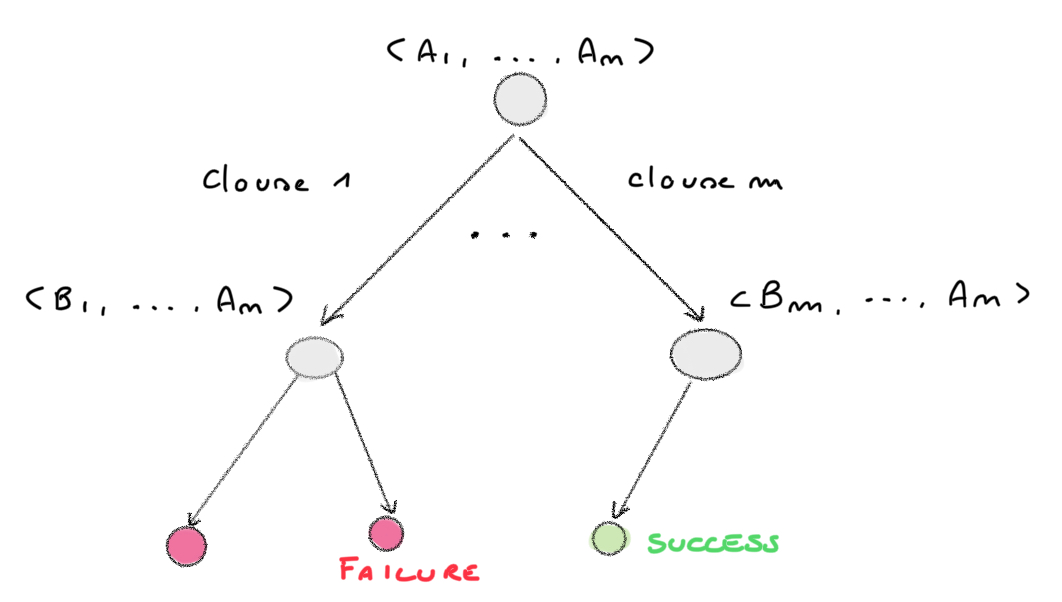
\includegraphics[width=0.75\linewidth]{unfold_tree}
\end{center}

The logical view of this rule is called resolution, which is a simpler proof
system than natural deduction and has only one rule:
$$\begin{prooftree}
    \hypo{R\lor A}\hypo{R'\lor \neg A}
    \infer2{R\lor R'}
\end{prooftree}$$
where $R$ and $R'$ are disjunction of literals and $A$ is an atomic
formula.

The idea is to work by contradiction, i.e. to use refutation: theory
united with negated consequence must be unsatisfiable.

The procedure is as follows:
\begin{enumerate}
    \item Transform all formulas into disjunction of literals (i.e.
        clauses).
    \item Add the negation of what we want to prove to the set of clauses.
    \item Apply the resolution rule.
    \item Stop when the empty clause is derived (i.e. the contradiction, i.e.
        false).
\end{enumerate}
\begin{example}
    Suppose we want to prove that $B$ is a logical consequence of $F=\{A\to
    B,A\}$. We proceed as follows:
    \begin{enumerate}
        \item First, we transform formulas in $F$ into clausal form:
            $$F=\{\neg A\lor B, A\}$$
        \item Then, we add negation of what we want to prove to $F$
            $$F=\{\neg A\lor B,A,\neg B\}$$
        \item We apply resolution:
            $$\begin{prooftree}
                \hypo{\neg A\lor B}\hypo{A}
                \infer2{B}\hypo{\neg B}
                \infer2{\square}
            \end{prooftree}$$
        \item Having obtained the empty clause, we conclude that $F$ is
            inconsistent and, therefore $F\models B$.
    \end{enumerate}
\end{example}
What we have shown applies to resolution for propositional logic; for FOL, the
idea remains the same. However, transforming FOL formulas into clauses is more
complex, and the resolution rule involves unification due to the presence of
variables.
While resolution is sound and complete for both propositional logic and FOL,
the order in which clauses are selected during resolution can, in some
instances, either prevent us from obtaining the empty clause or result in
indefinite creation of new clauses, never reaching the empty clause. This
shows the semi-decidability in FOL.
\subsection{Prolog}
In Prolog there is no iteration, but you can get iterative behaviour through
recursion.
\paragraph{Syntax}
\begin{itemize}
    \item Variables: \texttt{X,Y} (Upper case initial)
    \item Constants: \texttt{alice,a} (Lower case initial)
    \item Functions: \texttt{father(X)} 
    \item Predicates: \texttt{brother(X,Y)} 
    \item Facts: \texttt{head.}
    \item Rules: \texttt{head :- body.}
    \item Lists: A recursive data structure, based on the concept of cons
        lists, that is either empty or consists
        of two parts: a head and a tail (has to be a list). The \texttt{|}
        separates the head and the tail parts. 
        \begin{verbatim}
            '[|]'
            /   \
           1   '[|]'
               /   \
              2   '[|]'
                  /   \
                 3     []
        \end{verbatim}
        The following are lists:
        \begin{verbatim}
[] empty list
[a | [b | []]] or [a, b]
[a | [b | [c | []]]] or [a, b, c]
[[] | []] or [[]]
[[a | []] | [b | []]] or [[a], b]
        \end{verbatim}
        \begin{itemize}
            \item \textbf{member}
                \begin{verbatim}
% base case
member(X, [X | _]) % first element
% recursively check on the tail
member(X, [_ | Tail]) :- member(X, tail) 
                \end{verbatim}
            \item \textbf{length} 
                \begin{verbatim}
% base case
length([], 0).
% _ anonymous variable
length([_ | Tail], N) :- length(Tail, NT), N is NT+1.
                \end{verbatim}
            \item \textbf{append} 
                \begin{verbatim}
% base case
append([], L, L) 
append([H | T], L2, [H | NewTail]) :- 
    append(Rest1, L2, NewTail)
                \end{verbatim}
                \begin{itemize}
                    \item the recursion case, which reduces the first list by
                        one element and attempts to append \texttt{L2} to it
                        again. This process repeats until the first list is
                        empty, triggering the base case.
                    \item as the recursion unwinds, \texttt{NewTail} is built
                        up backward.
                \end{itemize}
                \begin{example}
                   \begin{verbatim}
?- append([1, 2, 3], [4, 5, 6], Result).
Result = [1, 2, 3, 4, 5, 6].

% Breaking down the recursion:
append([1, 2, 3], [4, 5, 6], Result).
H = 1, T = [2, 3], L2 = [4, 5, 6]
append([2, 3], [4, 5, 6], NewTail). 
H = 2, T = [3], L2 = [4, 5, 6]
append([3], [4, 5, 6], NewTail).
H = 3, T = [], L2 = [4, 5, 6]
% Base case reached, NewTail is [4, 5, 6]
append([], [4, 5, 6], NewTail).
                   \end{verbatim} 
                \end{example}
        \end{itemize}
\end{itemize}
In imperative programming languages, the position of a variable in an
assignment operation matters: if a variable is on the right side, its value is
accessed, and if it's on the left side, a value is assigned to it. This means
you cannot use the same operation for both input and output simultaneously.
However, in Prolog, it's possible to compute arguments as both input and
output depending on how the call is specified. This flexibility is due to
Prolog use of unification, which is \textbf{bidirectional}, unlike the one-way
assignment in imperative languages.
\begin{figure}[!ht]
    \centering
    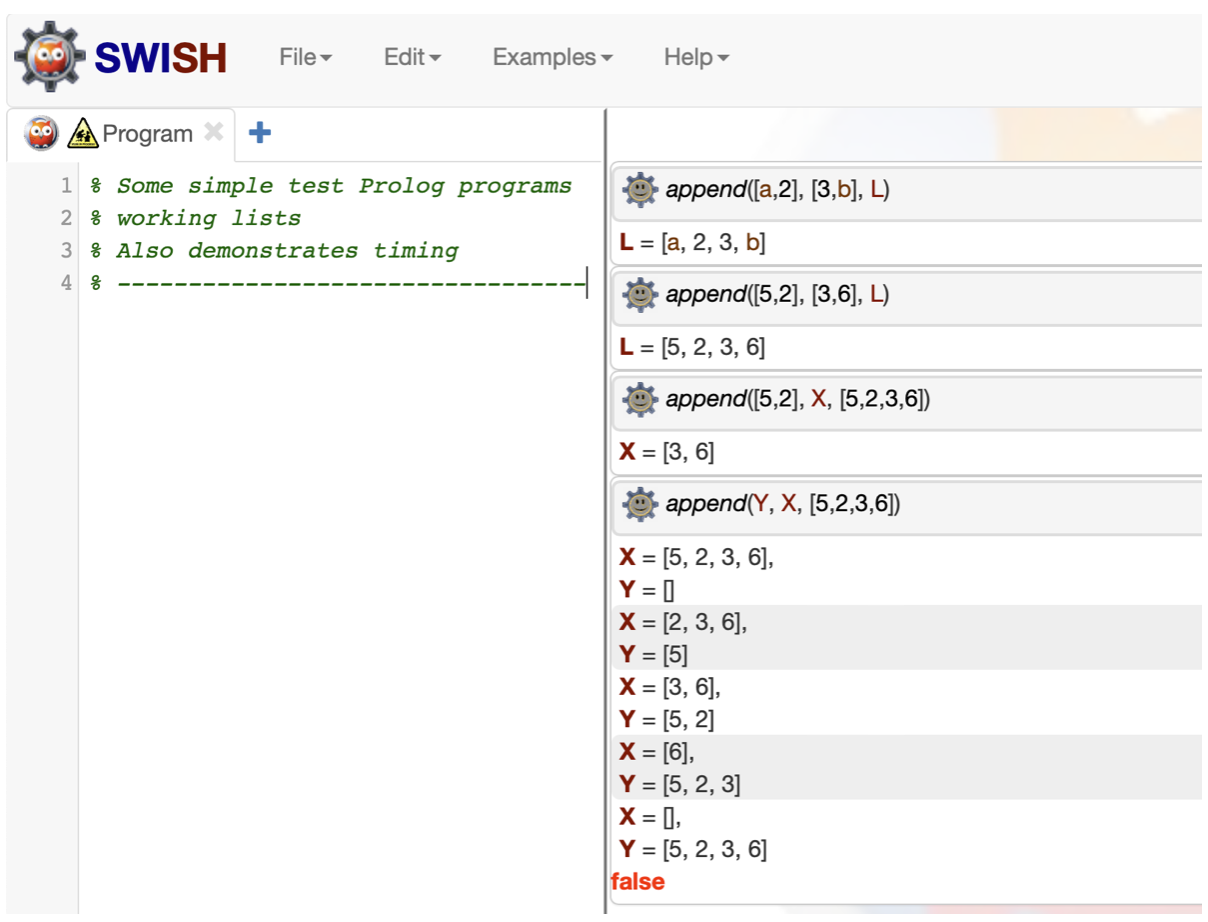
\includegraphics[width=\linewidth]{prolog_bidirectional}
    \caption{Bidirectional argument passing}
\end{figure}
\paragraph{Arithmetic.} In Prolog, integers and floating-point numbers are
constants. There are several math operators predefined as function symbols
(\texttt{+,-,*,\,div,mod}).

To evaluate arithmetic expressions, Prolog uses the predicate \texttt{X
{\color{red}is} Expression}, where \texttt{X} will be instantiated to the
value of \texttt{Expression}. 
\begin{example}
    \texttt{X is 2 + 3} will evaluate the expression 2 + 3 and unify X with the result, 5.
\end{example}
Variables in \texttt{Expr} \underline{must be already instantiated} at the
moment of evaluation.
\begin{example}
    \begin{verbatim}
p(X) :- Y is 3+5, X is Y. 
?- p(X).
X=8

p(X):-X is Y,Y is 3+5.
?- p(X).
error
    \end{verbatim}
\end{example}
Expressions can be compared using relational operators such as
\texttt{=:=,=\=,>,<,>=,=<} to evaluate their values.
\begin{example}
    Count the number of leaves of binary tree.
    \begin{verbatim}
  P <-     P <-     P <- Internal nodes  X <- Leaf
 / \      / \      / \                  / \
L   R    L  nil   nil R               nil nil
    \end{verbatim}
    First of all, how we represent a binary tree?
    I can use a function symbol, 
    \texttt{tree(P, L, R)}, and so can be used as term for another predicate.
    Now, I want to construct a predicate which given a tree counts the number
    of leaves of tree.
    \begin{verbatim}
tree_count(nil, 0)
tree_count(tree(_, nil, nil), 1)
tree_count(tree(_, L, R), N) :-
    tree_count(L, N1),
    tree_count(R, N2),
    N is N1 + N2
    \end{verbatim}
\end{example}
\paragraph{The predicate ! (cut).} The search strategy of the Prolog interpret
attempts to inspect the \underline{entire search tree}. To modify this
behavior, we can use the predicate cut (\texttt{!}) which can be inserted into
the body of any clause. When evaluated, it make some choices as definite and
non-backtrackable, thus allowing us to prune part of the search tree.
\begin{example}
    Consider the clause:
    \begin{verbatim}
       p :- q, r !, s.
    \end{verbatim}
    The choices made in the evaluation of goal \texttt{q} are definite. If
    \texttt{s} fails, Prolog will not backtrack to try to find another
    solution for either \texttt{q} or \texttt{r} but will fail immediately.
\end{example}
\begin{example}
    \begin{center}
        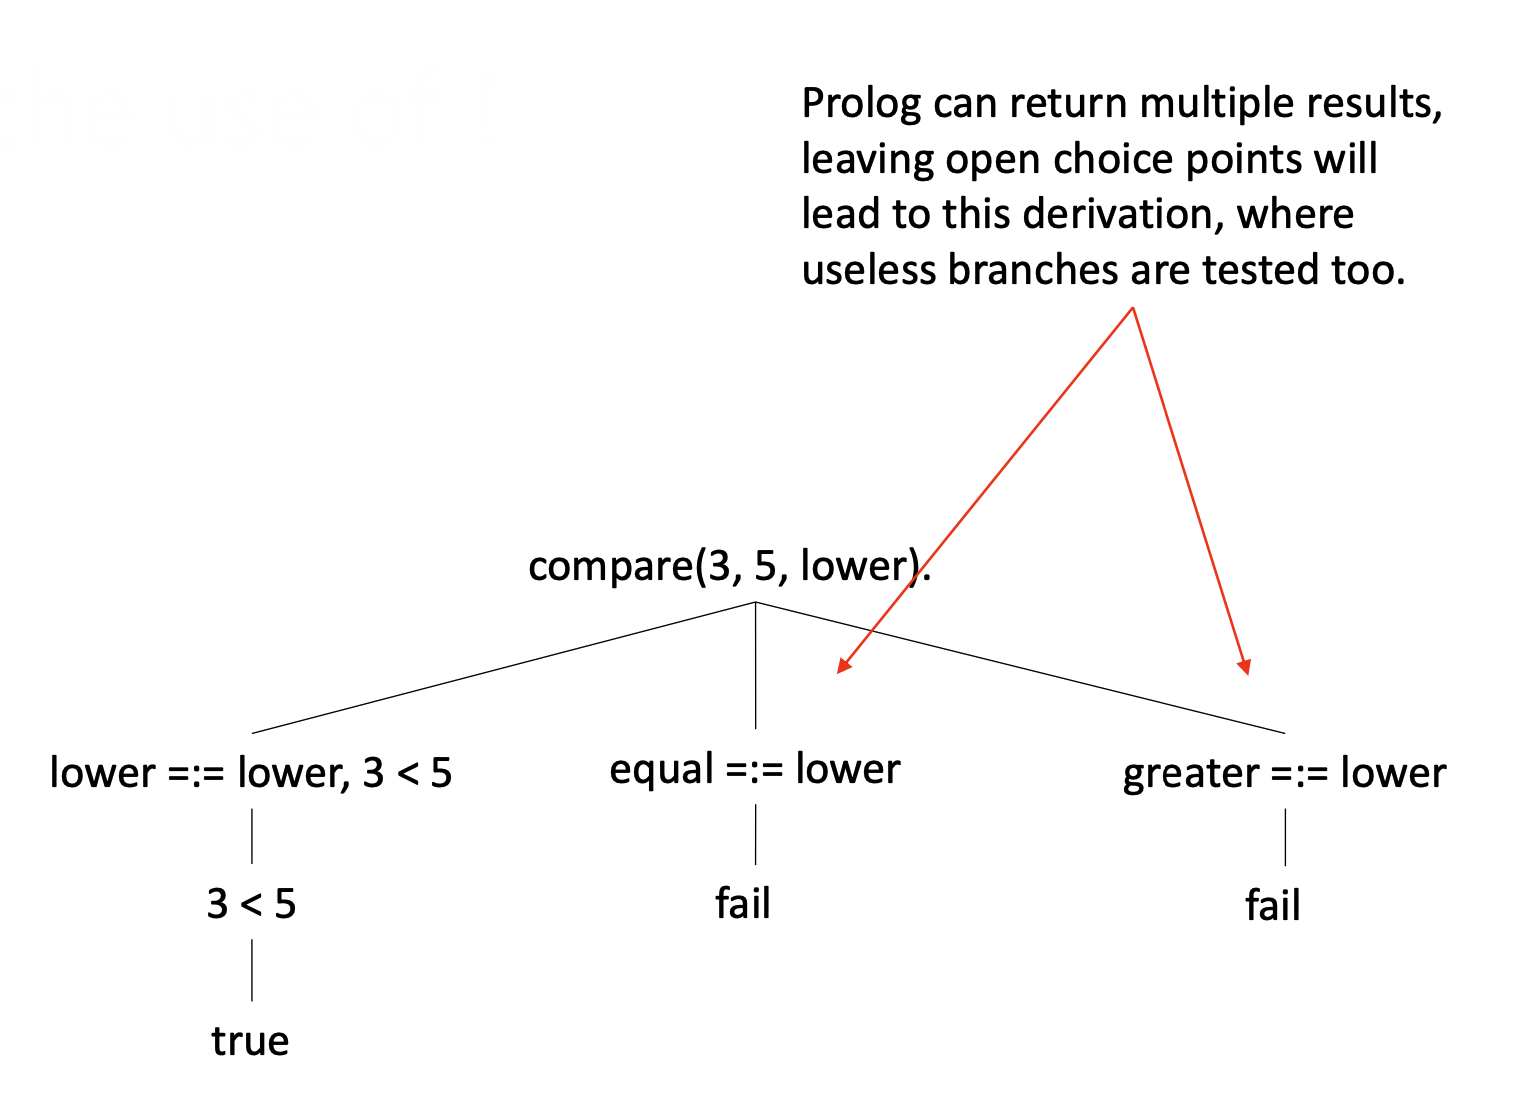
\includegraphics[width=0.75\linewidth]{compare_nocut}
    \end{center}
   \begin{verbatim}
compare(X, Y, lower) :- X < Y.
compare(X, Y, equal) :- X =:= Y.
compare(X, Y, greater) :- X > Y.

?- compare(3, 5, lower).
   \end{verbatim} 
    \begin{center}
        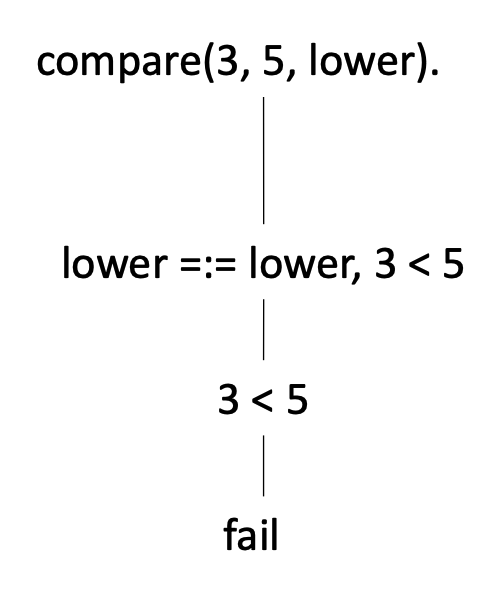
\includegraphics[width=0.25\linewidth]{compare_cut}
    \end{center}
   \begin{verbatim}
compare(X, Y, lower) :- X < Y, !.
compare(X, Y, equal) :- X =:= Y, !.
compare(X, Y, greater) :- X > Y.

?- compare(3, 5, lower).
   \end{verbatim} 
\end{example}
\begin{example}
    \begin{center}
        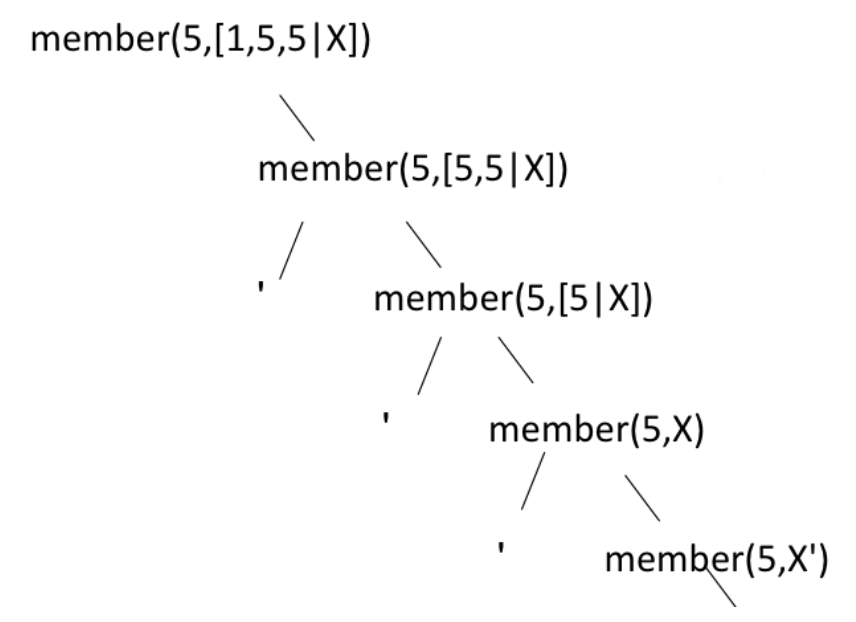
\includegraphics[width=0.75\linewidth]{member_nocut}
    \end{center}
   \begin{verbatim}
member(X, [X|_]). 
member(X,[-|L]) :- member(X,L).
   \end{verbatim}
   Each time Prolog finds a 5, and since \texttt{X} is an unbound variable, it
   means Prolog explores an infinite number of possible lists where 5 is a
   member, leading to an infinite number of solutions.
    \begin{center}
        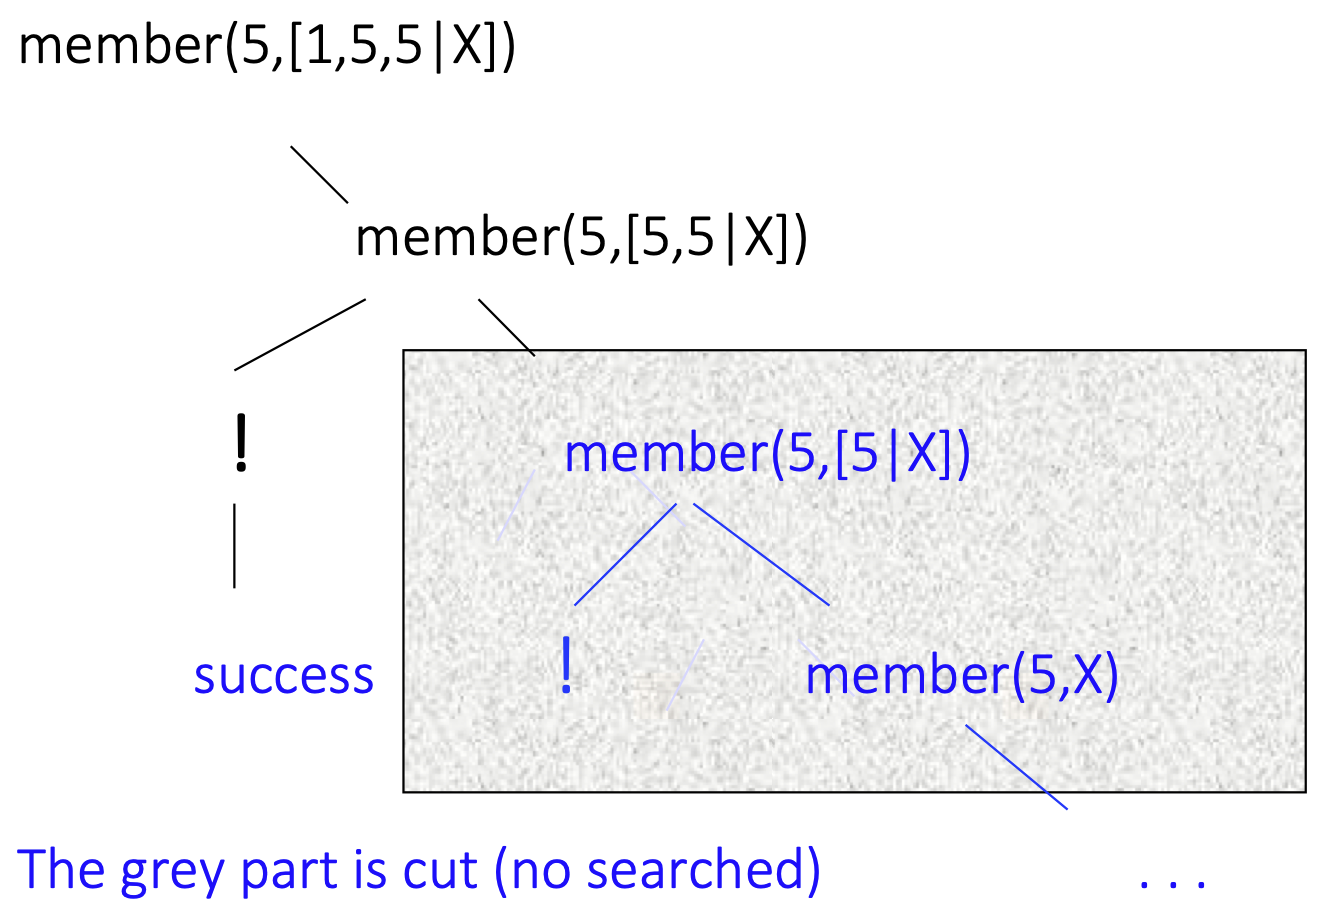
\includegraphics[width=0.75\linewidth]{member_cut}
    \end{center}
   \begin{verbatim}
member(X, [X|_]) :- !. 
member(X,[-|L]) :- member(X,L).
   \end{verbatim} 
\end{example}
\begin{example}
    The following code shows how to achieve the logic of \texttt{if
    then else} using the cut operator:
    \begin{verbatim}
p(X) :- a(X), !, b.
p(X) :- c.
    \end{verbatim}
\end{example}
\cleardoublepage
\section{Constraint programming}

In constraint programming, the goal is to create a model of the problem
through the use of a predefined set of constraints (equations). These
constraints can be either global, supplied by external sources, or custom,
defined by the programmer themselves. Once the problem has been modeled, a
predefined solver is employed to find a solution for us.

\begin{center}
    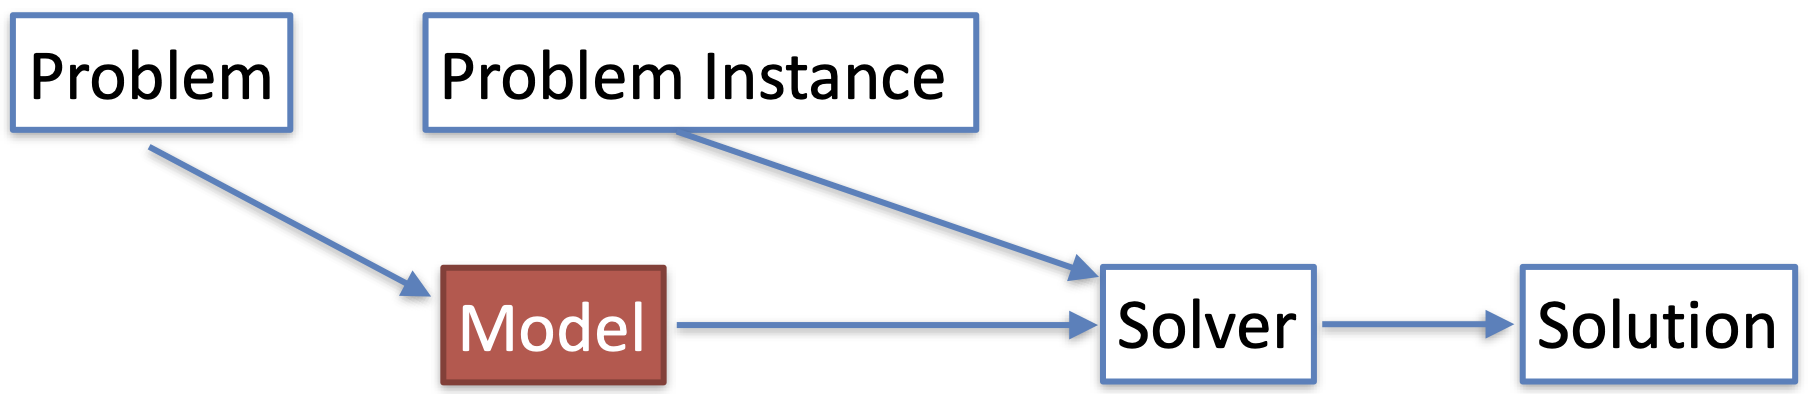
\includegraphics[width=0.95\linewidth]{cp_problem_solving}
\end{center}

There are two main classes of problems:
\begin{Definition}{Constraint Satisfaction Problems (CSP)}{}
    A CSP is defined by:
    \begin{itemize}
        \item a finite set of variables $\{X_1,\ldots,X_n\}$ 
        \item a set of possible values (Domain) for these variables
            $D(X_1),\ldots, D(X_n)$
        \item a set of constraints $\{C_1,\ldots,C_n\}$
    \end{itemize}
    A solution to a CSP is an assignment to all the variables that satisfies
    the constraints.

\end{Definition}
Similar to how a predicate is evaluated under an interpretation in FOL, a
constraint is satisfied if a pair of variables meets a defined meaning.
Specifically, the meaning of a constraint is given by specifying a set of
values that satisfy the relation. If a pair of variables belongs within this
set, the constraint is thereby satisfied.
\begin{Definition}{Constraint Optimization Problems (COP)}{}
    A COP is a CSP plus a function $f$ which expresses some cost. A solution
    to a COP is those values that optimizes this cost function $f$.
\end{Definition}
\newpage
We have two main families of constraint languages, to which we add constraints
(and the relative solvers):
\begin{itemize}
    \item \textbf{Constraint Logic Programming}
    \item \textbf{Imperative languages with constraints}
\end{itemize}
\subsection{Constraint Logic Programming}
\begin{Definition}{Alphabet}{}
    The alphabet is an extension of that used in logic
    programming~\ref{fol_alphabet}, augmented with symbols specific to
    constraints. Within this framework, a constraint can be seen as:
    \begin{itemize}
        \item an atomic constraint, which is an expression
            $c(t_1,\ldots,t_n)$ with $n\geq0$ terms as its arguments.
        \item a conjuction of constraints.
    \end{itemize}
    Additionally, CLP supports \textit{First-Order Constraint Theory}, which
    provides the possibility of defining the semantics of a constraint by
    allowing the programmer to introduce a set of axioms.
\end{Definition}
\paragraph{Syntax}
\begin{center}
   \begin{bnf}
        $A,B$ : Atom ::= $p(t_1,\ldots,t_n),\ n\geq0$ ;;
        $C,D$ : Constraint ::= $c(t_1,\ldots,t_n)\mid C\land D,\ n\geq0$;;
        $G,H$ : Goal ::= $\top \mid \perp\mid A\mid C\mid G\land H$ ;;
        $K$ : CL Clause ::= $A\leftarrow G$ ;;
        $P$ : CL Program ::= $K_1\ldots K_m,\ m\geq0$ ;;
   \end{bnf} 
\end{center}
In simpler terms, in the body of the clauses we can have constraints.

\begin{example}
    ``Send+More=Money" is puzzle where each letter represents a unique digit
    from 0 to 9. The goal is to find a digit for each letter such that when
    you add the numbers SEND and MORE together, they equal the number MONEY.
{\small
    \begin{verbatim}
[S,E,N,D,M,O,R,Y] = [9,5,6,7,1,0,8,2]

           SEND
           9567
        +  MORE
           1085 
          _____
        = MONEY
          10652
    \end{verbatim}
    \begin{verbatim}
:- use_module(library(clpfd)).

send([S,E,N,D,M,O,N,E,Y]) :-
    gen_domains([S,E,N,D,M,O,N,E,Y], 0..9),
    S #\=0, M #\= 0,
    all_distinct([S,E,N,D,M,O,R,Y]),
        1000*S + 100*E + 10*N + D 
        + 1000*M + 100*O + 10*R + E
        #= 10000*M + 1000*O + 100*N + 10*E + Y,
    labeling([],[S,E,N,D,M,O,R,Y]).

gen_domains([],_).
gen_domains([H|T],D) :- H in D, gen_domains(T,D).
    \end{verbatim}
}
    \begin{itemize}
        \item Check each element in the list to take
            a value from 0 to 9;
        \item Check that M and S are different from 0;
        \item Check all variables are distinct from one another;
        \item Check the sum holds, considering the positional encoding
            for each digit.
        \item Ground variables with values;
    \end{itemize}
\end{example}
The above example might seem Prolog, but not exactly. In pure Prolog, as we
have said, variables must be grounded with arithmetic Prolog built-ins, so we
cannot proceed as described in the code. We must move the \texttt{labeling}
line below \texttt{gen\_domains}. However, doing so means that every time one
of these conditions does not hold, it backtracks to find another solution
through different variable choices. This approach is impracticable for our
problem.

Luckily, the \texttt{clpfd} library allows us to use constraints in Prolog and
provides a substitute for Prolog arithmetic built-ins by simply prefixing them
with a \texttt{\#}. In this case, we are allowed to use constraints on
variables that are not grounded and structure the program as described above.
The key point here is to first accumulate the constraints and afterward ground
the variables with values. The constraints prune the search tree
\underline{before} actively do the search. In other words, they limit the
number of branches that could exist. Thus, a problem that may seem
impracticable can become easy to resolve.
\paragraph{Semantics.} Constraint Logic Programming has a transition system
similar to the one observed in logic programming, as previously discussed
(\ref{unfold_logic}), with some minor differences:
\begin{itemize}
    \item \textbf{Unfold}: Given $\langle A\land G, C\rangle$, the result of
        computation here is represented by a constraint rather than a
        substitution. We select a compatible clause with a matching predicate
        name and unifiable $B\leftarrow H$, from program $P$. In the unfold
        step $\langle A\land G, C\rangle \mapsto\langle H\land G,(B=A)\land
        C\rangle$, we replace the call with the body of the clause as usual.
        However, instead of performing unification directly, we add equations
        representing the constraint that perform the unification implicitly.
        By solving these equations, we achieve the same result as the
        unification, even though these equations are not solved.
    \item \textbf{Solve}: we simplify the constraints accumulated so far by
        combining them and applying them to narrow down the possible values of
        the variables $(C\land D_1)\leftrightarrow D_2$.
\end{itemize}
\subsection{MiniZinc}
\paragraph{Syntax}
\begin{itemize}
    \item Each expression terminates with \texttt{;}
    \item Variable domain and array index domain must all be specified
    \item Index array starts from 1 not 0
    \item Comments \texttt{\%} 
    \item Range \texttt{0..10}
    \item Arithmetic Operators \verb|+,-,*,/,^,=,!=|
    \item Logical Operators \verb|\/,/\,->,!|
    \item We specify data for parameters in separate files ending with
        \texttt{.dzn} extension. To execute the program, we can use the
        following command:
        \begin{verbatim}
minizinc program.mzn data.dzn
        \end{verbatim}
\end{itemize}
MiniZinc allows the programmer to specify:
\begin{itemize}
    \item \textbf{Parameters}: we instantiate the values of these based on the
        current problem instance.
        \begin{verbatim}
[domain]:[parameter name]
        \end{verbatim}
    \item \textbf{Variables}: variables that will be instantiated by the
        solver.
        \begin{verbatim}
var [domain]:[variable name]
        \end{verbatim}
    \item \textbf{Constraints}: rules that a solution must respect.
        \begin{verbatim}
constraint [expression]
        \end{verbatim}
        Global constraints:
        \begin{verbatim}
include "global.mzn";
all_different()
all_equal()
        \end{verbatim}
    \item \textbf{Arrays}: can be either a set of parameters or variables.
        \begin{verbatim}
array[index_domain] of [domain]
array[index_domain] of var [domain]
        \end{verbatim}
    \item \textbf{Aggregation functions}: \verb|sum, product, min,|
        \verb|max, forall, exists|
        \begin{verbatim}
% sum of all the elements in array
sum(array_x) 
% sum of elements from 1 to 3 of array
sum(i in 1..3)(array_x[i])
% first 3 elements in array are different
forall (i,j in 1..3 where i < j) (array_x[i] != array_x[j])
        \end{verbatim}
\end{itemize}
A MiniZinc program includes \texttt{solve} keyword, followed by
\texttt{satisfy}, \texttt{maximize}, or \texttt{minimize} to indicate the kind
of problem. For the cases of \texttt{maximize} and \texttt{minimize}, an
objective function must be also specified. Without \texttt{solve} keyword, it
is implicitly a satisfaction problem.
\begin{example}
    \begin{center}
        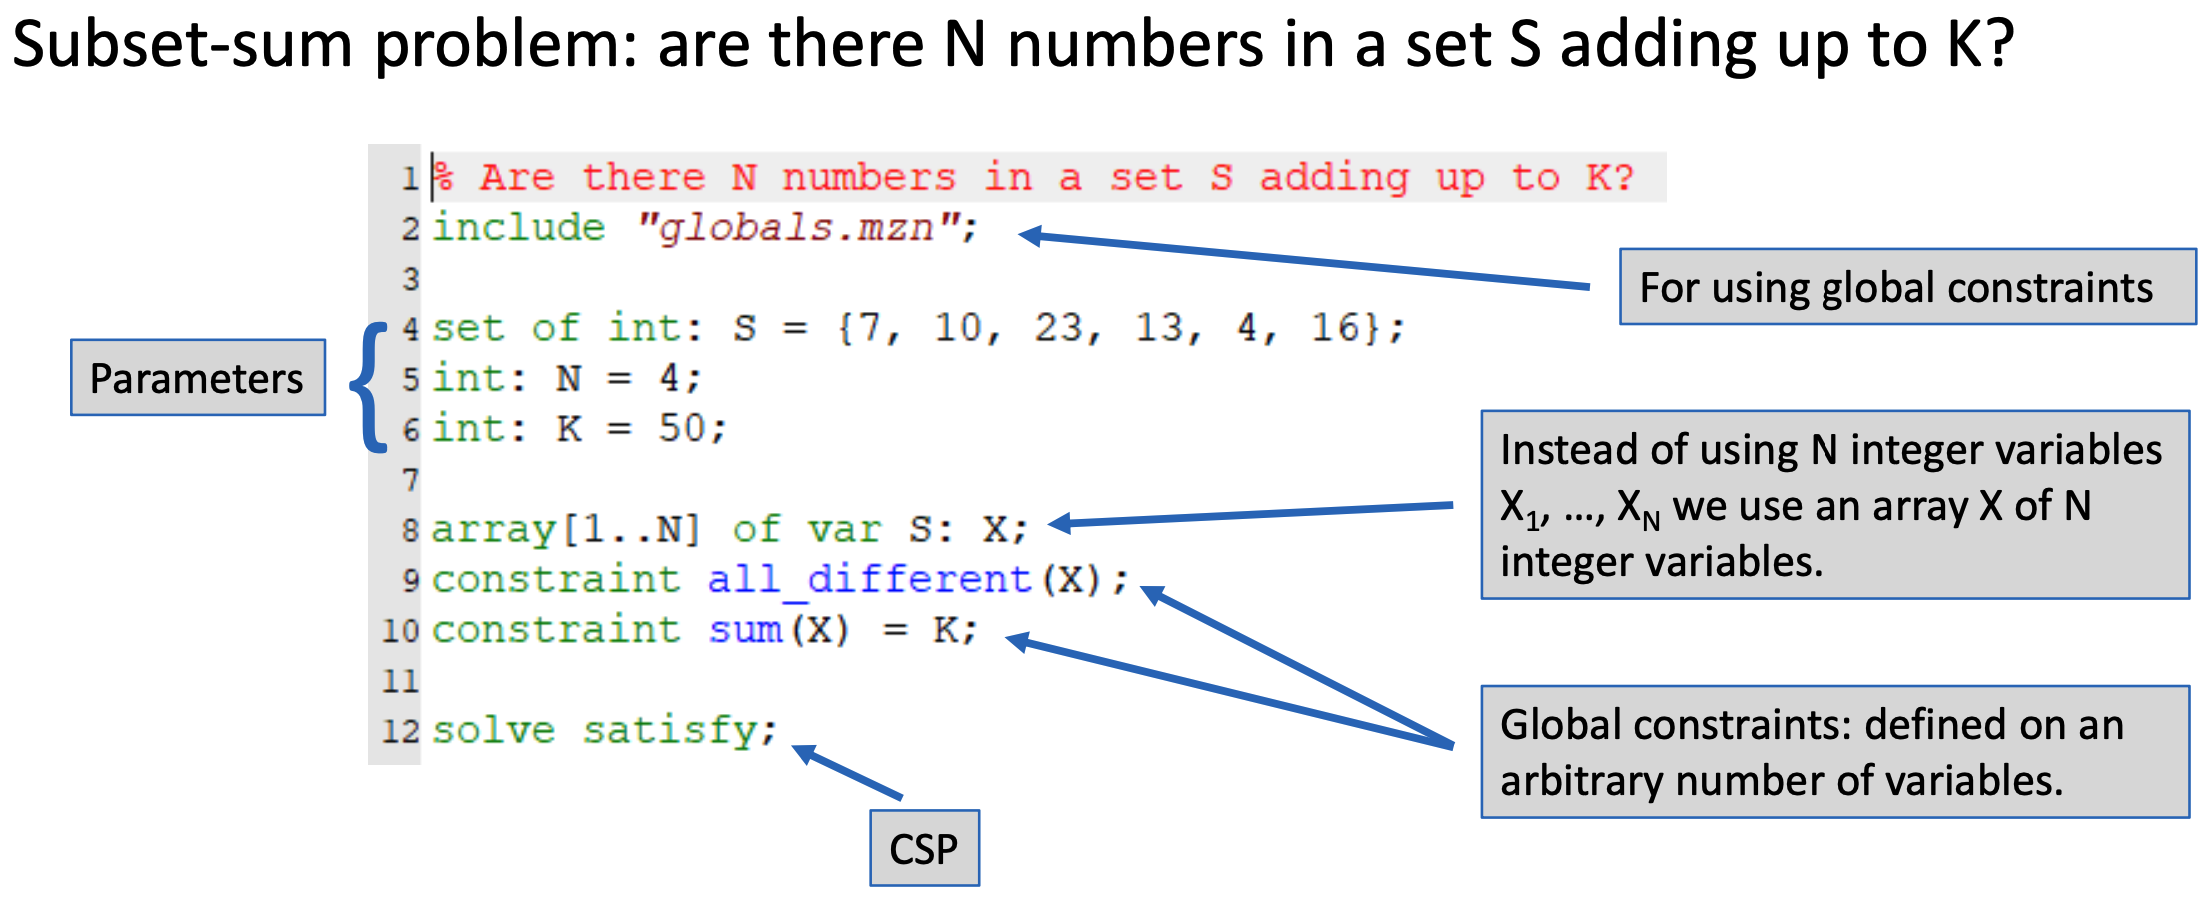
\includegraphics[width=\linewidth]{subset_sum}
    \end{center}
\end{example}
\begin{example}
   \begin{center}
       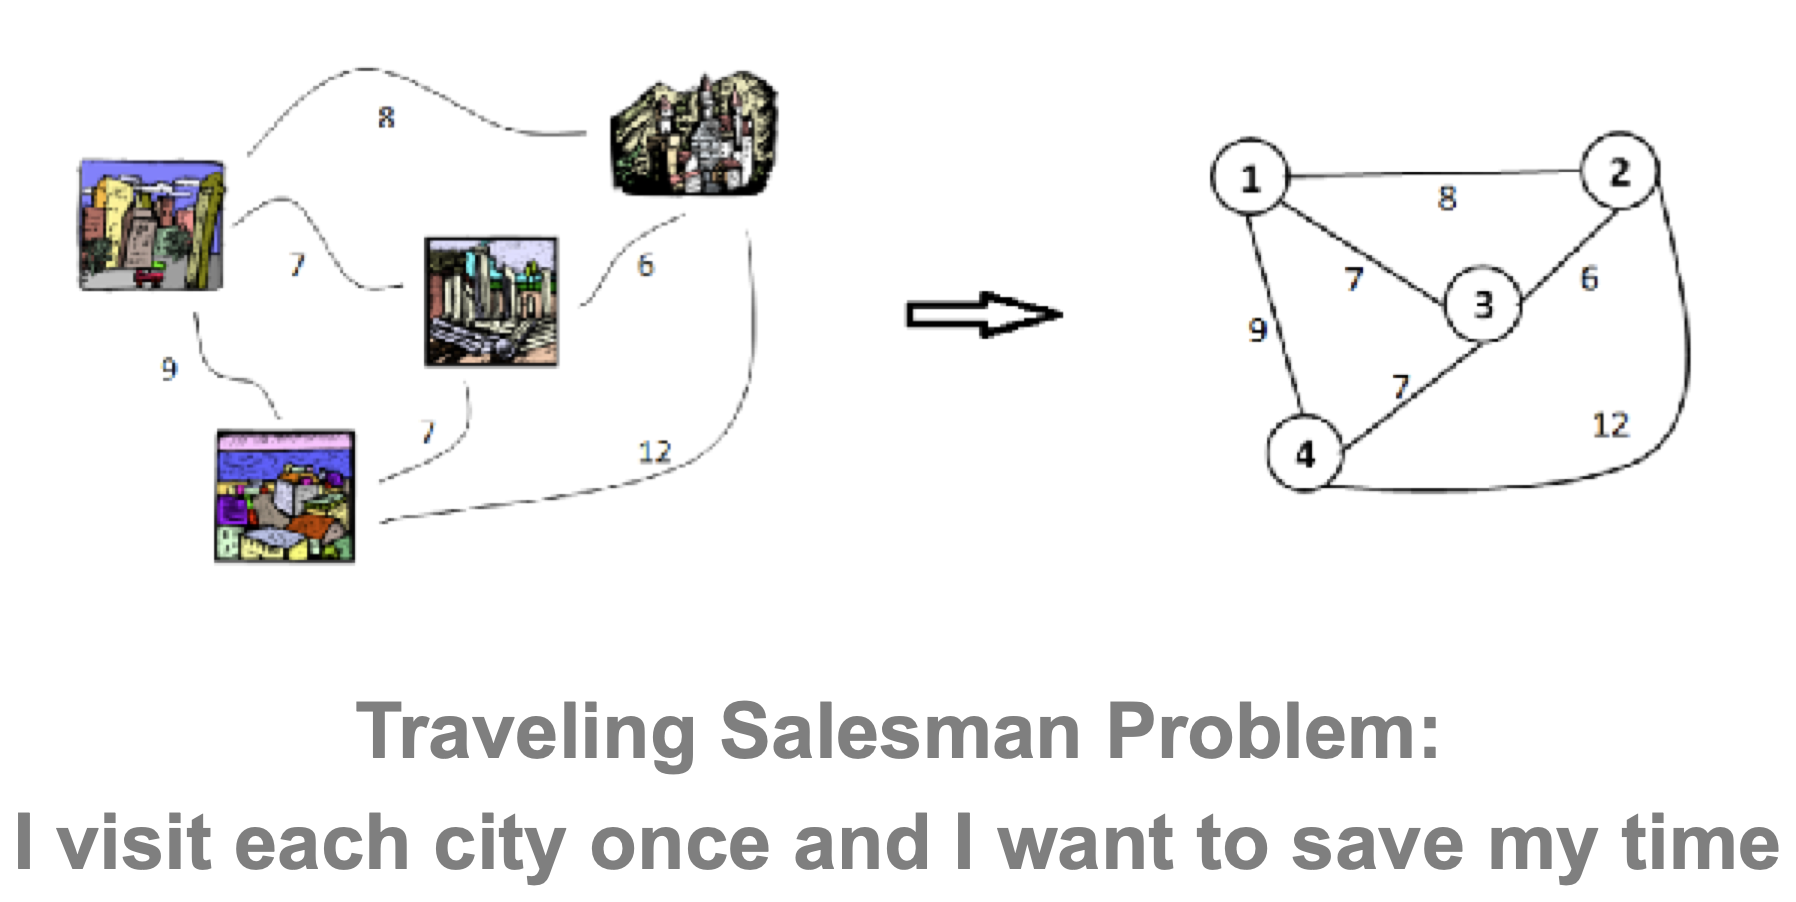
\includegraphics[width=\linewidth]{travel_salesman_problem}
   \end{center} 
   \begin{center}
       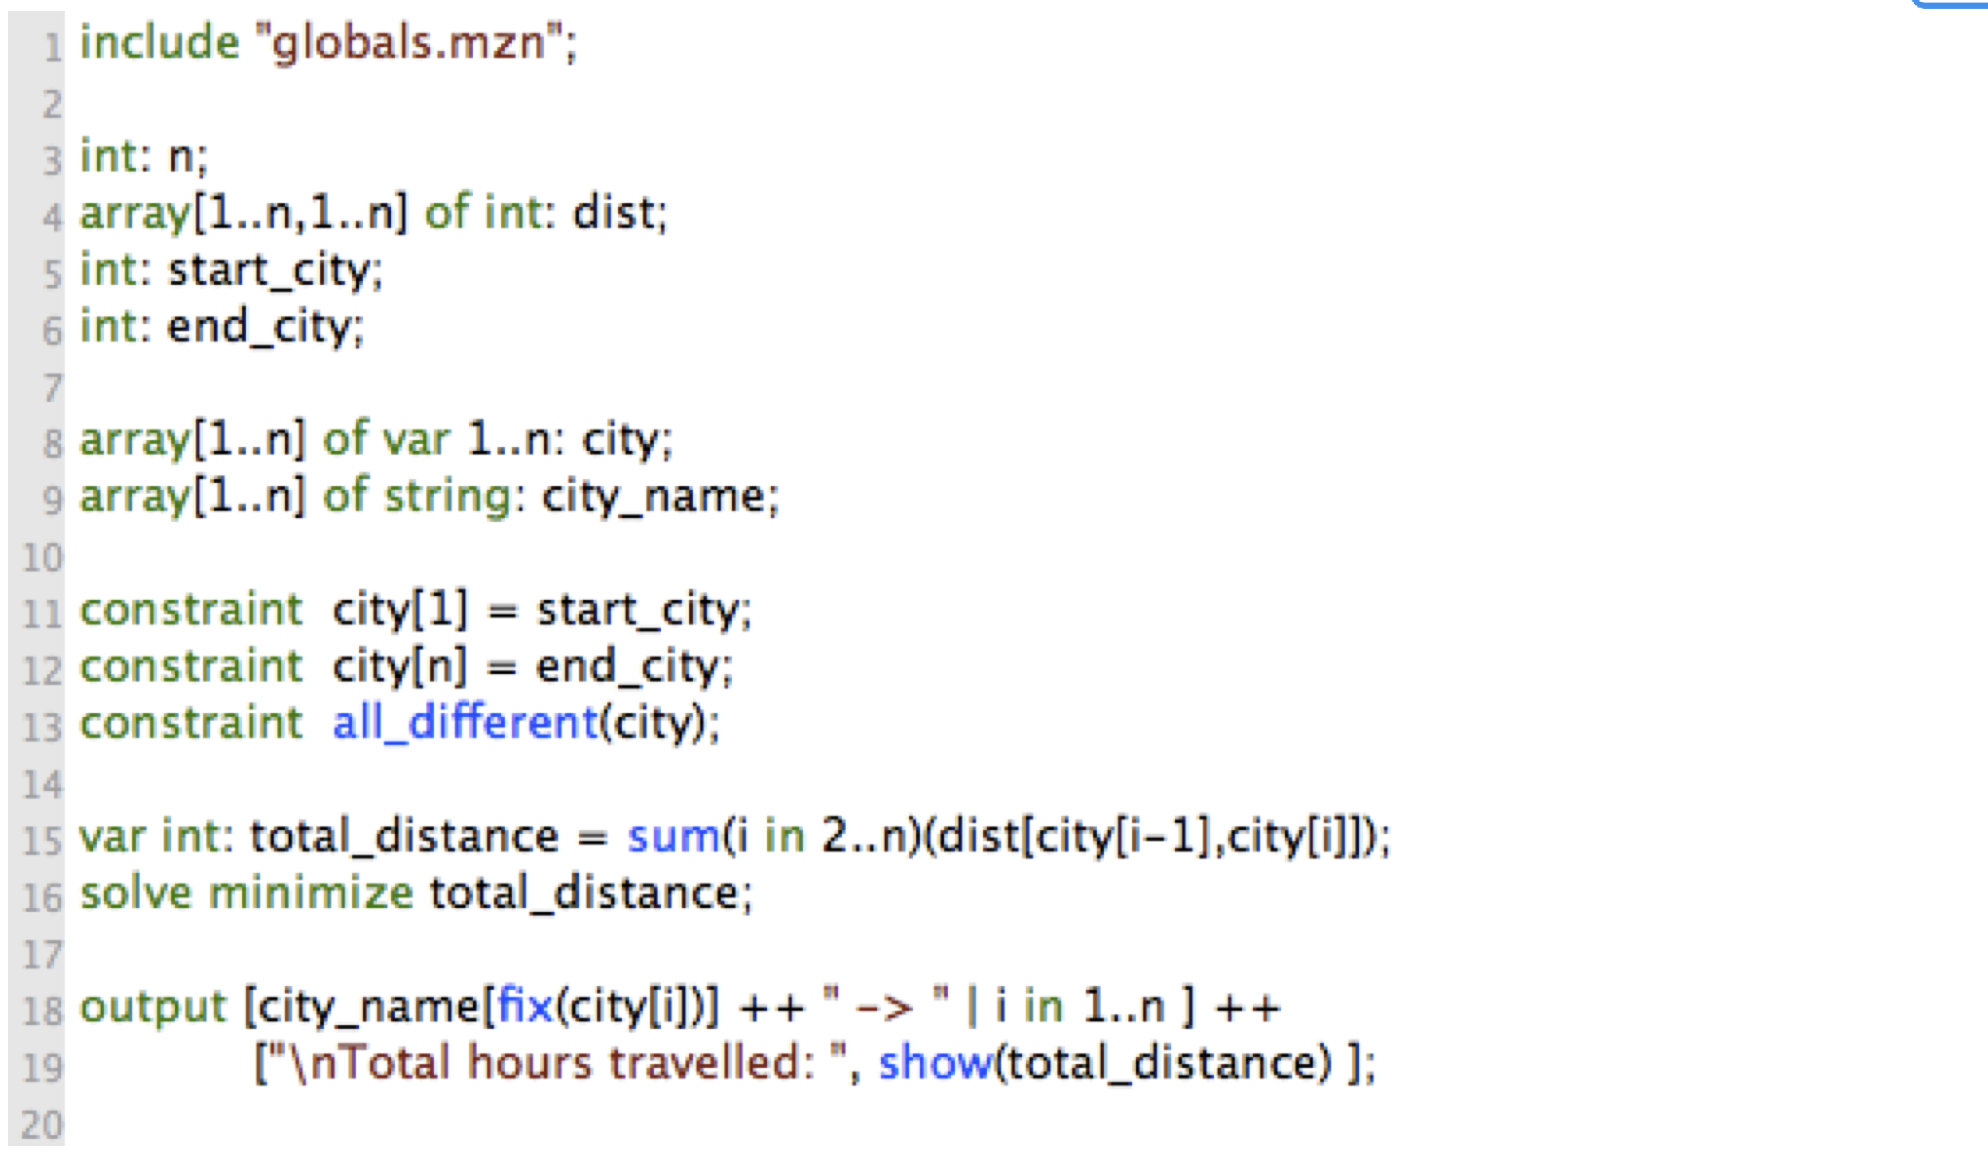
\includegraphics[width=\linewidth]{travel_salesman_minizinc}
   \end{center}
\end{example}
\end{document}